\documentclass[../Report.tex]{subfiles}


\begin{document}


\chapter{Einführung}
\label{chap:einfuehrung}
Mit Barrier Bucket (BB) RF Systemen sollen am neu entstehenden Synchrotron SIS100 oder im Experimentier Speicherring (ESR) am GSI Helmholtzzentrum unterschiedliche longitudinale Manipulationen an Teilchenstrahlen vorgenommen werden. Der dazu notwendige Spannungspuls hat die in \figref{fig:BB_req} dargestellte Form. Wenn die Wiederholfrequenz des Spannungspulses gleich der Umlauffrequenz ist, so führt dies zu einer stationären Potentialbarriere im Phasenraum. Diese Barrieren können dazu verwendet werden, den Strahl longitudinal einzuschließen und ermöglichen somit varialble Bruchlängen. Unterscheiden sich Wiederholfrequenz des Spannungssignals und Umlauffrequenz, so gewegt sich die Barriere im Phasenraum ("moving barrier") und ermöglicht Kompression/Dekompression der Bunches.\\ Eine Herausforderung dieser Systeme liegt darin, eine hohe Qualität des Pulses am Gap der Kavität zu erzeugen, um unerwünschte Effekte auf den Strahl zu verhindern. Laut Spezifikation für das EST System müssen die Nachschwinger nach dem Einzelsinus beispielsweise kleiner als 2,5\% von $\hat{U}_{BB}$ sein.
\begin{figure}[H]
  \centering
  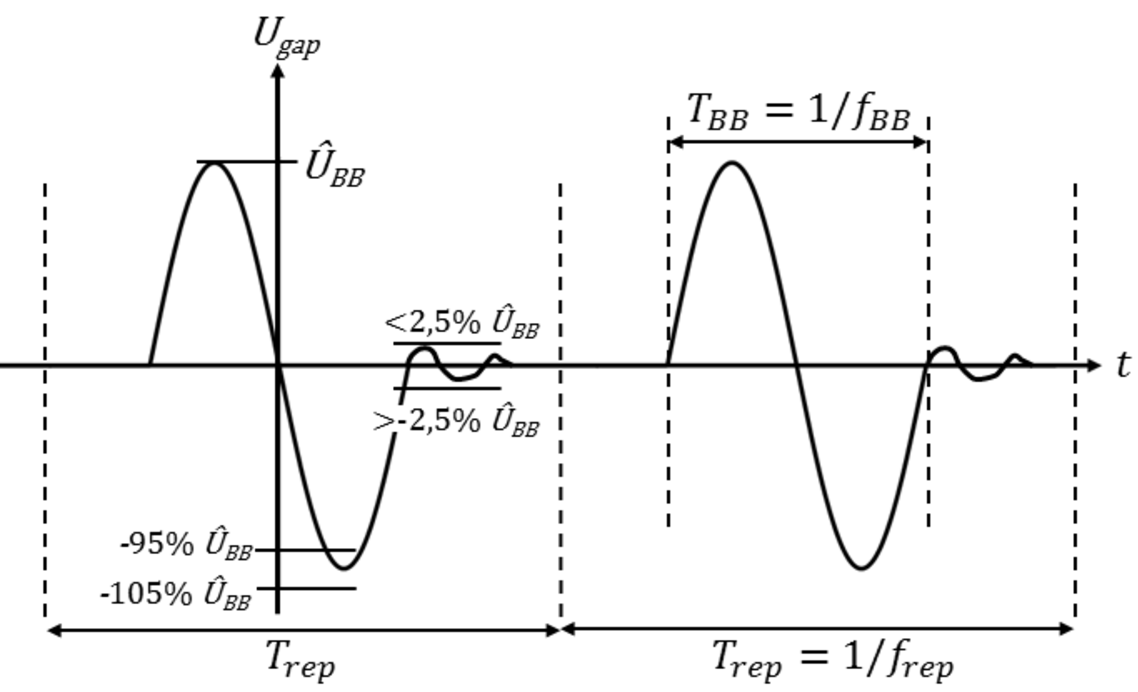
\includegraphics[width=0.7\textwidth]{eps/BB_req.pdf}
  \caption{Ausgangssignal}
  \label{fig:BB_req}
\end{figure}

Dabei wird im Folgenden $f_{rep}$ für die Wiederholfrequenz des Spannungssignals verwendet. Die Barrier Bucket Frequenz $f_{BB}$ bestimmt die Breite der Potential Barriere. Für die Messungen in diesm Projektseminar wurden ${f_{rep} = 900 \si{\kilo \hertz}}$ und ${f_{BB} = 5 \si{\mega \hertz}}$ verwendet.


\section[Modell und Konvention]{Versuchsaufbau und Modell}
\label{sec:einf.modell_BB}
Der Prototyp des ESR BB besteht aus einem Funktionsgenerator (Keysight 3600A series 2-channel ($50\Omega $) AWG), einem Verstärker (AR1000A225) und der Breitband Ringkern-Kavität. Der Versuchsaufbau ist in \figref{fig:Aufbau} gezeigt. Ein Messablauf ist in \figref{fig:Messung} als Flow Chart Diagramm dargestellt.\\
Dabei kann angenommen werden, dass sich das System bis $\hat{U}_{BB} = 550V$ annähernd linear verhält und durch die Übertragungsfunktion $\Hcompl$ beschrieben werden kann. Eine mathematische Modellierung ist ebenfalls in \figref{fig:Aufbau} gegeben, bei der zur linearen Übertragungsfunktion $\Hcompl$ noch eine nichtlineare Kennlinie enthalten ist. Die Größen werden im nächsten Abschnitt erklärt.
\begin{figure}[H]
	\centering
	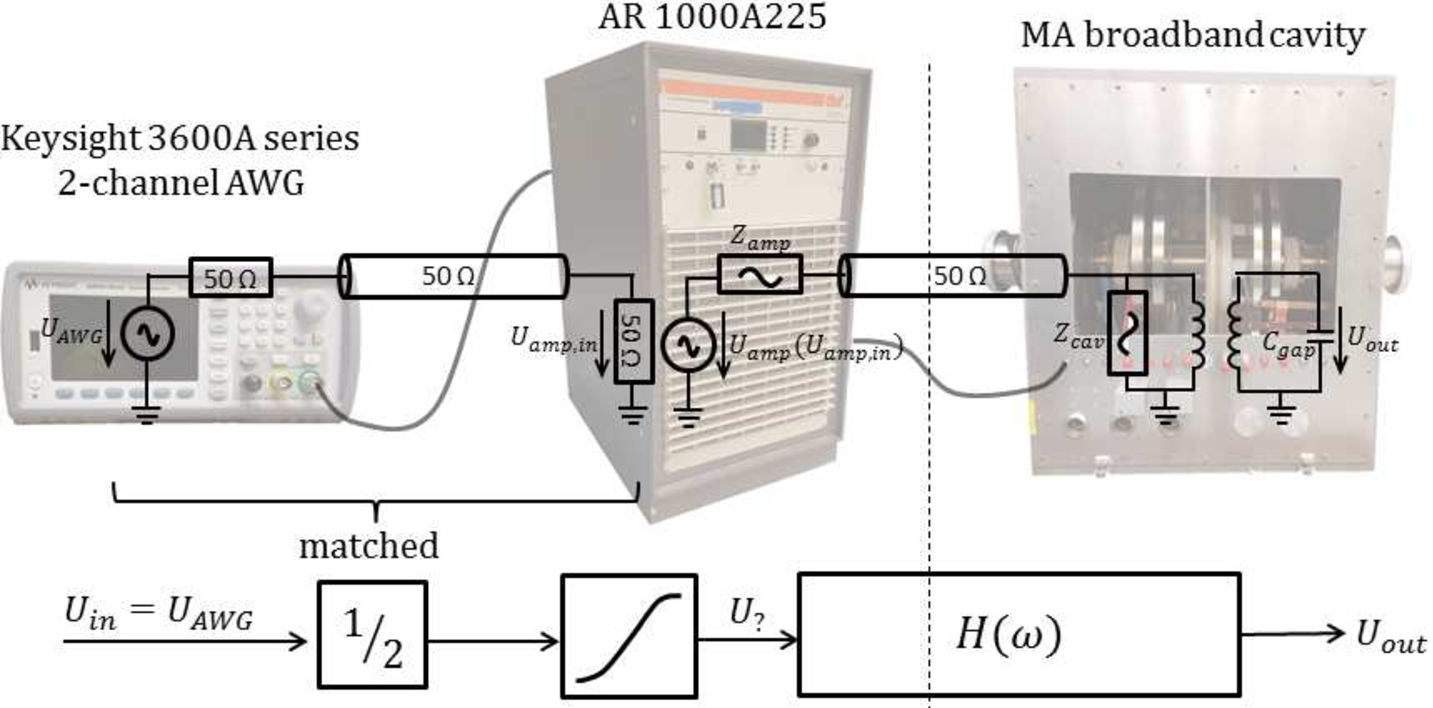
\includegraphics[width=0.7\textwidth]{eps/Aufbau.pdf}
	\caption{Versuchsaufbau und Modell siehe \cite{harzheim}}
  	\label{fig:Aufbau}
\end{figure}

\begin{figure}[H]
\centering

\tikzstyle{decision} = [diamond, draw, fill=blue!20, 
    text width=4.5em, text badly centered, node distance=3cm, inner sep=0pt]
\tikzstyle{block_g} = [rectangle, draw, fill=green!20, 
    text width=5em, text centered, rounded corners, node distance=3cm, minimum height=4em]
\tikzstyle{block_b} = [rectangle, draw, fill=blue!20, 
    text width=5em, text centered, rounded corners, node distance=5cm, minimum height=4em]
\tikzstyle{block_r} = [rectangle, draw, fill=red!20, 
    text width=5em, text centered, rounded corners, node distance=3cm, minimum height=4em]
\tikzstyle{line} = [draw, -latex']
\tikzstyle{cloud} = [draw, ellipse,fill=red!20, node distance=5cm,
    minimum height=2em]
    
\begin{tikzpicture}[node distance = 2cm, auto]
    % Place nodes
    \node [block_g] (init) {Programm};
    \node [block_b, below of=init] (kav) {Ringkern-Kavität};
    \node [block_b, left of=kav] (amp) {Verstärker};
    \node [block_b, right of=kav] (gap) {Gap-\newline spannungs- \newline teiler 1:800};
    \node [cloud, left of=init] (AWG) {AWG};
    \node [cloud, right of=init] (DSO) {DSO};
    
    % Draw edges
    \draw [->] (init) -- node {$\Uin$} (AWG);
    \draw [->] (AWG) -- node [near start]{} (amp);
    \draw [->]
  	(AWG) -- ++(0,13mm)   -- node {ch1} ++(100mm,0) -- (DSO);
    \draw [->] (amp) -- (kav);
    \draw [->] (kav) -- (gap);
    \draw [->] (gap) -- node {ch3, ch4} (DSO);
    \draw [->] (DSO) -- node {$\Uout$} (init);
\end{tikzpicture}
\caption{Ein Messdurchlauf}
  	\label{fig:Messung}
\end{figure}
Das berechnete Eingangssignal $\Uin$ wird an das AWG übergeben davon wird es zum einen an das Oszilloskop geleitet und zu anderen an den Verstärker. Der Gapspannungsteiler hat ein Verhältnis von 1:800 dabei ergibt sich die Ausgangsspannung $\Uout$ als die Differenz der Kanäle 3 und 4. Es muss darauf geachtet werden, dass alle Eingang des Oszilloskops auf hoch-ohmig eingestellt sind, um Schäden am Gerät zu verhindern. Dabei müssen die Leitungen von der Kavität mit einem T-Stück und einem $\SI{50}{\Omega}$ Widerstand abgeglichen sein. Die Ausgänge des AWG müssen auch auf $\SI{50}{\Omega}$ eingestellt werden.
\subsection{Hammerstein Modell}
\label{subsec:einf.modell_BB.hammerstein}
In \figref{fig:Hammerstein} sind alle verwendeten Größen dargestellt. $U_{in}$ ist die Eingangsspannung des Funktionsgenerators. Der erste Block in \figref{fig:Hammerstein} stellt die nichtlineare Modellierung dar. Die Spannung $U_{?}$ ist eine rein virtuelle Größe und kann wie in \eqref{eq:Uquest} aus der Eingangsspannung über die Koeffizienten $a_n$ berechnet werden. Bei der Potenzreihe hatte $N = 3$ in der MATLAB Implementierung schon gute Ergebnisse geliefert und wurde daher weiterhin so verwendet. Die nichtlinearen Kennlinie im Folgenden nur noch als $K$ bezeichnet, wird als Look-Up Tabelle im Programm hinterlegt. Die Spannung $U_{out}$ ist die Gapspannung in der Kavität.
\begin{figure}[H]
	\centering
	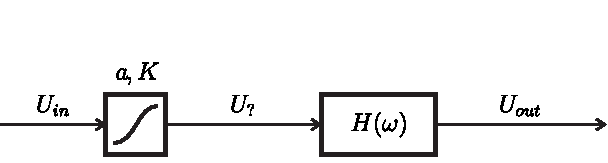
\includegraphics[width=0.5\textwidth]{eps/Hammerstein.pdf}
	\caption{Hammerstein Modell}
  	\label{fig:Hammerstein}
\end{figure}
\begin{align}
	U_?(t)=\sum_{n=1}^N \, a_n \, \left[ U_{in}(t) \right]^n
	\label{eq:Uquest}
	\qquad
	\Uout \oft = \mathscr{F}^{-1} \left\{ \Hcompl \ofomega \cdot \Uinc \ofomega \right\}
\end{align}

\section{Motivation}
\label{sec:einf.motivation}
Das Hammerstein Modell wurde bis auf die Berechnung von $K$ schon erfolgreich in Python implementiert. Dabei sei auf das Projektseminar \cite{PJS_Denys} verwiesen. Deshalb lag unsere Motivation darin, dieses Modell in Python zu vervollständigen, um dann einen möglichen Optimierungsansatz aufzustellen.


\section{Aufgabenstellung}
\label{sec:einf.aufgabe}
Im Rahmen dieses Projektseminars sollte eine iterative Optimierung der Vorverzerrung auf Basis einer Hammersteinmodellierung in Python implementiert werden. Dabei sollte das Tool die nichtlineare Kennlinie $K$ und die Übertragungsfunktion $\Hcompl$ wechselseitig optimieren, wobei eine optimale Gewichtung der Parameter zur Optimierung noch nicht erreicht werden musste.
\end{document}